\documentclass{beamer}
\usepackage[frenchb]{babel}
\usepackage[utf8]{inputenc}
\usepackage[T1]{fontenc}
\usepackage{graphicx}
\usepackage{tikz}
\usepackage{subcaption}
\usetikzlibrary{arrows, decorations.markings}
\usetheme{Warsaw}


%%------Métadonnées------%%
\title{Formaliser le refactoring
\\ à l'aide de transformations de graphe}
\author{Alois Paulus}
\date{\today}


%%------Début du document------%%
\begin{document}

	%%------Page de titre------%%
	\begin{frame}
		\titlepage
		\vfill
		\begin{center}
			\vspace*{-3.5ex}
		\end{center}
	\end{frame}

	%%------Slide------%%
	\frame{\frametitle{Qu'est-ce que le refactoring?}

	\begin{quotation}
		"Le refactoring est un processus qui a pour objectif la transformation et l’amélioration du code source d’un logiciel.
		Le logiciel en question ne doit pas subir de régression au niveau fonctionnel mais doit gagner en performance et en évolutivité."
	\end{quotation}
	}

	%%------Slide------%%
	\frame{\frametitle{Pourquoi formaliser le refactoring}
	\begin{itemize}
		\item But
		\begin{enumerate}
			\item Possibilité d'utiliser ce modèle dans des outils de refactoring
			\item Supporter plusieurs langages de programmation
			\item Garantir la préservation du comportement du programme
		\end{enumerate}
	\end{itemize}
	}

	%%------Slide------%%
	\frame{\frametitle{Pertinence de l'emploi de graphe}

	\begin{itemize}
		\item Facilite l'intégration dans des outils de refactoring
		\item Transformation de graph pour représenter le refactoring
		\item Possède des propriétés mathématiques
	\end{itemize}
	}

	%%------Slide------%%
	\frame{\frametitle{Les différents types de graphe}

	\begin{itemize}
		\item Graphe de programme
		\item Graphe de type
		\item Graphe d'expression
	\end{itemize}

	}

	%%------Slide------%%
	\frame{\frametitle{Graphe de programme (1/3)}
	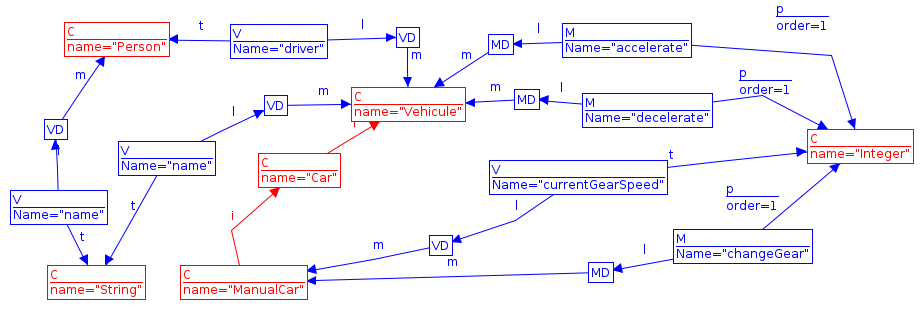
\includegraphics[width=\linewidth,height=\textheight,keepaspectratio]{slidesProgramGraph.png}
	}

	%%------Slide------%%
	\frame{\frametitle{Graphe de type (2/3)}
	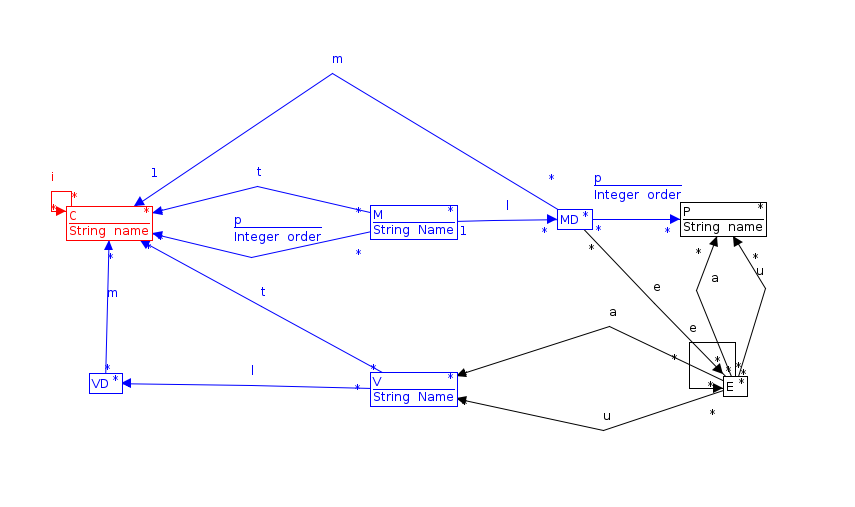
\includegraphics[width=\linewidth,height=\textheight,keepaspectratio]{typeGraph.png}
	}

	%%------Slide------%%
	\frame{\frametitle{Graphe d'expression (3/3)}
	\begin{tikzpicture}[->,>=stealth',shorten >=1pt,auto,node distance=3cm,
		thick, label distance=-1mm, label position=45, every label/.style={blue}]

		\node (rect) at (9.5,6) [draw,thick,minimum width=1cm,minimum height=0.5cm,label=2] (Fig1MD2) {MD};
		\node (rect) at (7,6) [draw,thick,minimum width=1cm,minimum height=0.5cm,label=1] (Fig1MD1) {MD};
		\node (rect) at (7,4) [draw,thick,minimum width=1cm,minimum height=0.5cm,label=4] (Fig1P) {P};
		\node (rect) at (9.5,4) [draw,thick,minimum width=1cm,minimum height=0.5cm,label=3] (Fig1E) {E};

		\node (rect) at (6.5,2) [draw,thick,minimum width=1cm,minimum height=0.5cm,label=2] (Fig2MD2) {MD};
		\node (rect) at (4,2) [draw,thick,minimum width=1cm,minimum height=0.5cm,label=1] (Fig2MD1) {MD};
		\node (rect) at (4,0) [draw,thick,minimum width=1cm,minimum height=0.5cm,label=4] (Fig2P) {P};
		\node (rect) at (6.5,0) [draw,thick,minimum width=1cm,minimum height=0.5cm,label=3] (Fig2E) {E};

		\node (rect) at (12.5,2) [draw,thick,minimum width=1cm,minimum height=0.5cm,label=2] (Fig3MD2) {MD};
		\node (rect) at (10,2) [draw,thick,minimum width=1cm,minimum height=0.5cm,label=1] (Fig3MD1) {MD};
		\node (rect) at (10,0) [draw,thick,minimum width=1cm,minimum height=0.5cm,label=4] (Fig3P) {P};
		\node (rect) at (12.5,0) [draw,thick,minimum width=1cm,minimum height=0.5cm,label=3] (Fig3E) {E};

		\path[every node/.style={font=\sffamily\small}]
		(Fig1MD2) edge [left] node [right] {e*} (Fig1E)
		(Fig1E) edge node {a{|}u} (Fig1P)
		(Fig1MD1) edge node {p} (Fig1P);

		\path[every node/.style={font=\sffamily\small}]
		(Fig2MD2) edge [left] node [right] {e*} (Fig2E)
		(Fig2E) edge node {u} (Fig2P)
		(Fig2MD1) edge node {p} (Fig2P);

		\path[every node/.style={font=\sffamily\small}]
		(Fig3MD2) edge [left] node [right] {e*} (Fig3E)
		(Fig3E) edge node {a} (Fig3P)
		(Fig3MD1) edge node {p} (Fig3P);
	\end{tikzpicture}
	}

	%%------Slide------%%
	\frame{\frametitle{Transformations de graphe (1/4)}
	\begin{itemize}
		\item Définir les conditions avant transformation
		\item Remplacement d'un sous graph par un autre sous graph
		\item Rediriger certaines arrêtes
	\end{itemize}
	}

	%%------Slide------%%
	\frame{\frametitle{Transformations de graphe : LHS / RHS et Préconditions (2/4)}
	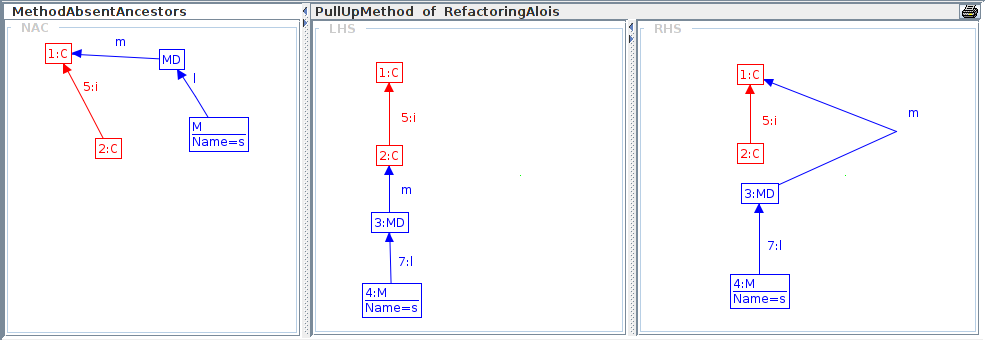
\includegraphics[width=110mm,scale=0.5,keepaspectratio]{full.png}
	}

	%%------Slide------%%
	\frame{\frametitle{Transformations de graphe : Application d'une transformation (3/4)}
	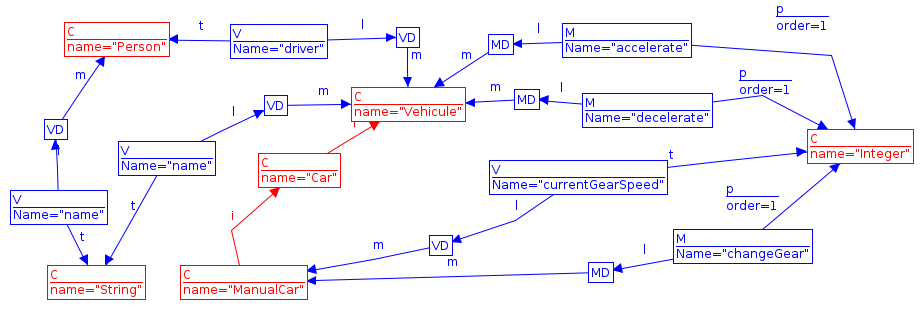
\includegraphics[width=\linewidth,height=\textheight,keepaspectratio]{slidesProgramGraph.png}
	}

	%%------Slide------%%
	\frame{\frametitle{Transformations de graphe : Application d'une transformation (4/4)}
	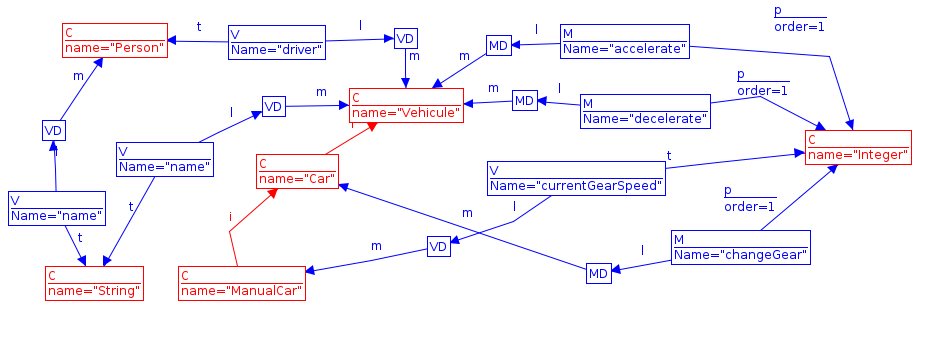
\includegraphics[width=\linewidth,height=\textheight,keepaspectratio]{afterTransfo.png}
	}

	%%------Slide------%%
	% \frame{\frametitle{Transformations de graphe : Redirection des arrêtes (5/5)}
	% \begin{tikzpicture}
	% 	\node[] at (1,5) {L};
	% 	\draw (2,4) ellipse (1cm and 0.5cm);
	% 	\node[] at (2,4) {V};
	%
	% 	\draw[->] (5,4) -- +(1,0);
	% 	\draw[->] (2,3) -- +(0,-1) node[anchor=west] {m};
	%
	% 	\node[] at (8,5) {R};
	% 	\draw (9,4) ellipse (1cm and 0.5cm);
	% 	\node[] at (9,4) {W};
	%
	% 	\draw[->] (9,3) -- +(0,-1) node[anchor=west] {n};
	%
	% 	\node[] at (0,1) {G};
	% 	\draw (2,0) ellipse (2cm and 1cm);
	% 	\draw (2,0) ellipse (1cm and 0.5cm);
	% 	\node[] at (2,0) {m(v)};
	%
	% 	\draw[->] (5,0) -- +(1,0);
	%
	% 	\draw (3.5,0) node[anchor=south] (e) {\textbullet};
	% 	\draw (2.5,0) node[anchor=south] (f) {\textbullet};
	%
	% 	\draw (0.5,0) node[anchor=south] (g) {\textbullet};
	% 	\draw (1.5,0) node[anchor=south] (h) {\textbullet};
	%
	% 	\draw[-latex] (e.west) to[out=90,in=70] (f.east);
	%
	% 	\draw[-latex] (h.west) to[out=70,in=90] (g.east);
	%
	% 	\node[] at (7,1) {H};
	% 	\draw (9,0) ellipse (2cm and 1cm);
	% 	\draw (9,0) ellipse (1cm and 0.5cm);
	% 	\node[] at (9,0) {n(w)};
	%
	% 	\draw (10.5,0) node[anchor=south] (a) {\textbullet};
	% 	\draw (9.5,0) node[anchor=south] (b) {\textbullet};
	%
	% 	\draw (7.5,0) node[anchor=south] (c) {\textbullet};
	% 	\draw (8.5,0) node[anchor=south] (d) {\textbullet};
	%
	% 	\draw[-latex] (a.west) to[out=90,in=70] (b.east);
	%
	% 	\draw[-latex] (d.west) to[out=70,in=90] (c.east);
	%
	% \end{tikzpicture}
	% }

	%%------Slide------%%
	\frame{\frametitle{Conservation du comportement(1/3)}
	\begin{itemize}
		\item Propriétés à préserver
		\begin{enumerate}
			\item Accès aux variables
			\item Mise à jour de variable
			\item Appel de méthode
		\end{enumerate}
	\end{itemize}

	}

	%%------Slide------%%
	\frame{\frametitle{Fonction de tracking(2/3)}
	\begin{center}
		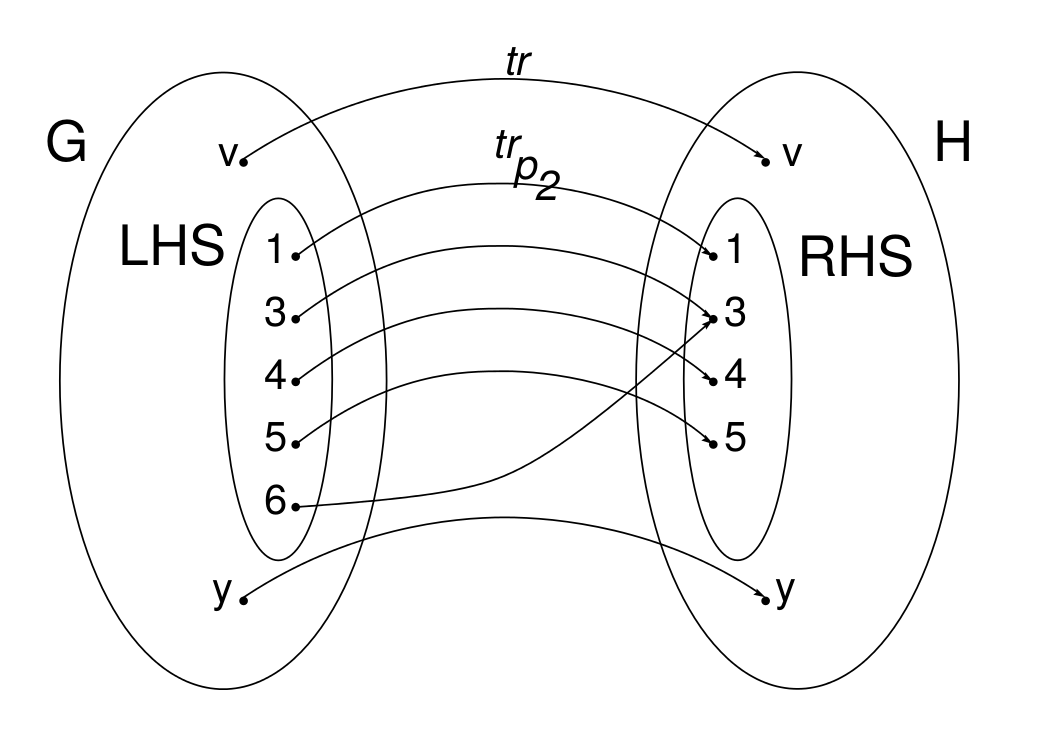
\includegraphics[width=100mm,keepaspectratio]{fonctionTrack.png}
	\end{center}
	}

	%%------Slide------%%
	\frame{\frametitle{Démonstration (3/3)}
	\tikzset{every picture/.append style={font=\tiny}}
	\begin{center}
		\begin{tikzpicture}[->,>=stealth',shorten >=1pt,auto,node distance=3cm,
			thick, label distance=-1mm, label position=45, every label/.style={blue}]

			\node [draw,thick,minimum width=1cm,minimum height=0.3cm,label=1] at (0,1.5)  (varLeft) {var V};

			\draw[thick,->] (1,1.5) -- (2,1.5);
			\node[red] at (1.5,1) {P1};

			\node (rect) at (3,2) [draw,thick,minimum width=1cm,minimum height=0.3cm,label=3] (setter) {Setter M};
			\node (rect) at (3,1) [draw,thick,minimum width=1cm,minimum height=0.3cm,label=4] (getter) {Getter M};
			\node (rect) at (5,1.5) [draw,thick,minimum width=1cm,minimum height=0.3cm,label=1] (varRight) {var V};

		\end{tikzpicture}
	\end{center}
	\begin{tikzpicture}[->,>=stealth',shorten >=1pt,auto,node distance=1cm,
		thick, label distance=-1mm, label position=45, every label/.style={blue}]
		\tikzstyle{EdgeStyle}=[bend left]

		\node at (0,1.5) [draw,thick, minimum width=1cm, minimum height=0.3cm,label=2] (setter) {Setter M};
		\node at (0,0) [draw,thick,minimum width=1cm,minimum height=0.3cm,label=3] (getter) {Getter M};
		\node at (2,1.5) [draw,thick,minimum width=1cm,minimum height=0.3cm,label=1] (varLeft) {var V};
		\node at (2,0) [draw,thick,minimum width=1cm,minimum height=0.3cm,label=0] (vdLeft) {VD};

		\draw[thick,->] (3,1) -- (4,1);
		\node[red] at (3.5,0.5) {P2};

		\node at (5,1.5) [draw,thick,minimum width=1cm,minimum height=0.3cm,label=4] (mdSetter) {MD};
		\node at (5,0) [draw,thick,minimum width=1cm,minimum height=0.3cm,label=2] (setter) {Setter M};
		\node at (7.5,1.5) [draw,thick,minimum width=1cm,minimum height=0.3cm,label=1] (varRight) {var V};
		\node at (7.5,0) [draw,thick,minimum width=1cm,minimum height=0.3cm,label=0] (vdRight) {VD};
		\node at (10,1.5) [draw,thick,minimum width=1cm,minimum height=0.3cm,label=5] (mdGetter) {MD};
		\node at (10,0) [draw,thick,minimum width=1cm,minimum height=0.3cm,label=3] (getter) {Getter M};

		\path[every node/.style={font=\sffamily\small}]
		(setter) edge [left] node [right] {l} (mdSetter)
		(getter) edge [left] node [right] {l} (mdGetter)
		(mdGetter) edge node {a} (varRight)
		(mdSetter) edge node {u} (varRight)
		(varLeft) edge [left] node [right] {l} (vdLeft)
		(varRight) edge [left] node [right] {l} (vdRight);
	\end{tikzpicture}

	\begin{table}
		\scriptsize
		\begin{tabular}{ | l | l |  l |}
			\hline production & arêtes entrantes & arêtes sortantes  \\ \hline
			P1 : & (\(a,1) {\rightarrow} (a,1)\) &  (\(t,1) {\rightarrow} (t,1),(1.p,2),(t,3)\)   \\ \hline
			& (\(u,1) {\rightarrow} (u,1)\) & \( (l,1) {\rightarrow} (l,1)\)  \\ \hline
			P2 : & \((a,1) {\rightarrow} (c,3)\) &  \((m,0) {\rightarrow} (m,0),(m,4),(m,5)\)    \\ \hline
			& (\(u,1) {\rightarrow} (c,2)\) &  \((t,1) {\rightarrow} (t,1)\)  \\ \hline
		\end{tabular}
	\end{table}

	}

	%%------Slide------%%
	\frame{
	\begin{center}
		\Large\textsc{Avez-vous des questions?}
	\end{center}
	}

\end{document}
